\section{First experiments}
\label{sec:exp1}

In the first set of experiments, we aim to compare our model with the errors made by measuring a well known object, shown in Figure \ref{fig:c5-cad}. The target was made with a \acs{CNC} machine with a precision of $0.1 \, mm$ with respect to all the measures reported in Figure \ref{fig:c5-cad-misure}. Our goal was to reach this measurement precision. \\

The point cloud obtained with our algorithm is shown in Figure \ref{fig:c5-profile_pixel}: the points are plotted in the world reference system, after that we have projected the laser spots, detected in the image.

\begin{figure}
  \begin{minipage}[c]{.44\textwidth}
    \centering
    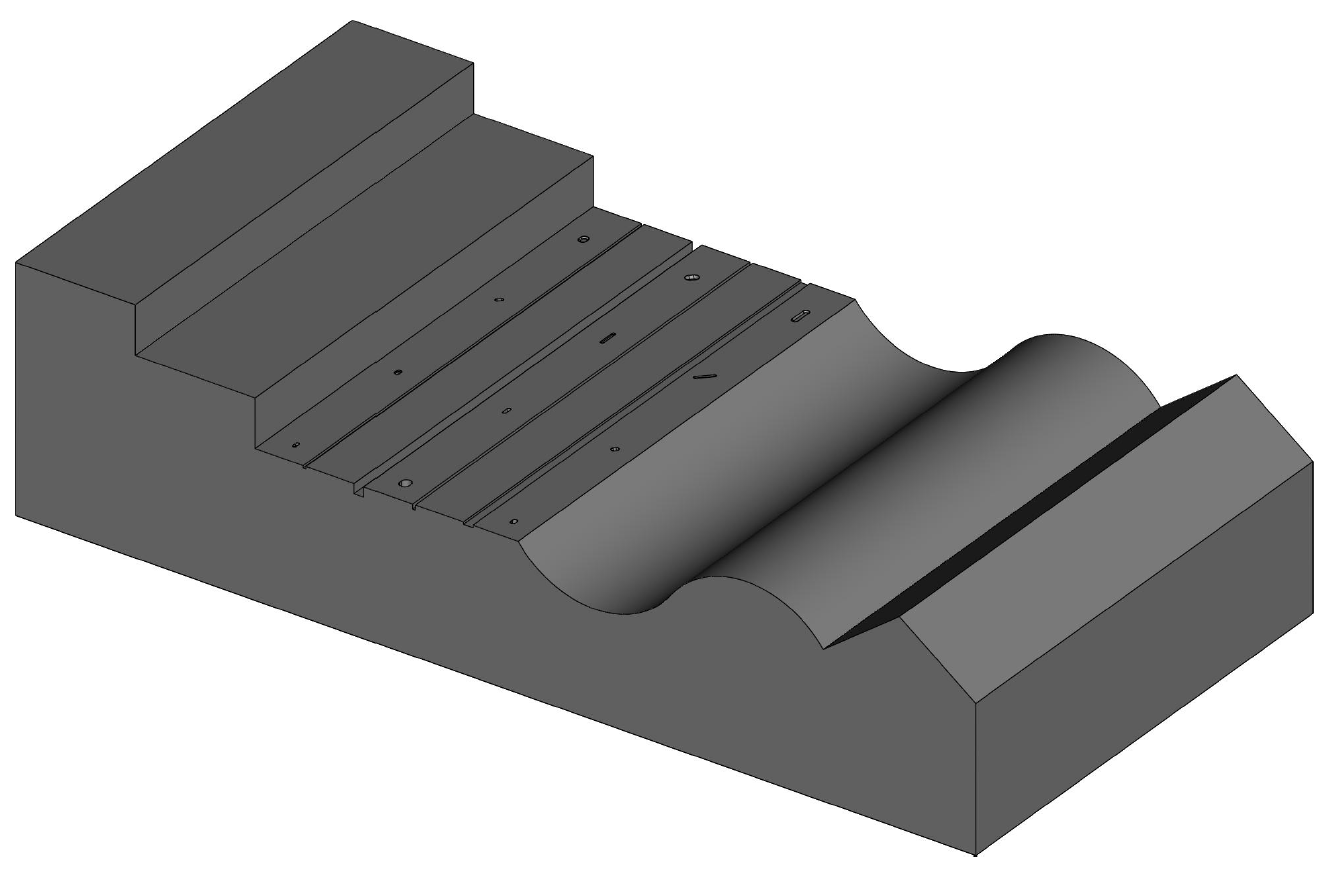
\includegraphics[width=\textwidth]{./images/analysis/t1/cad.png}
    \caption{CAD of the target \\ object}
    \label{fig:c5-cad}
  \end{minipage}
  \hfill
  \begin{minipage}[c]{.55\textwidth}
    \centering
    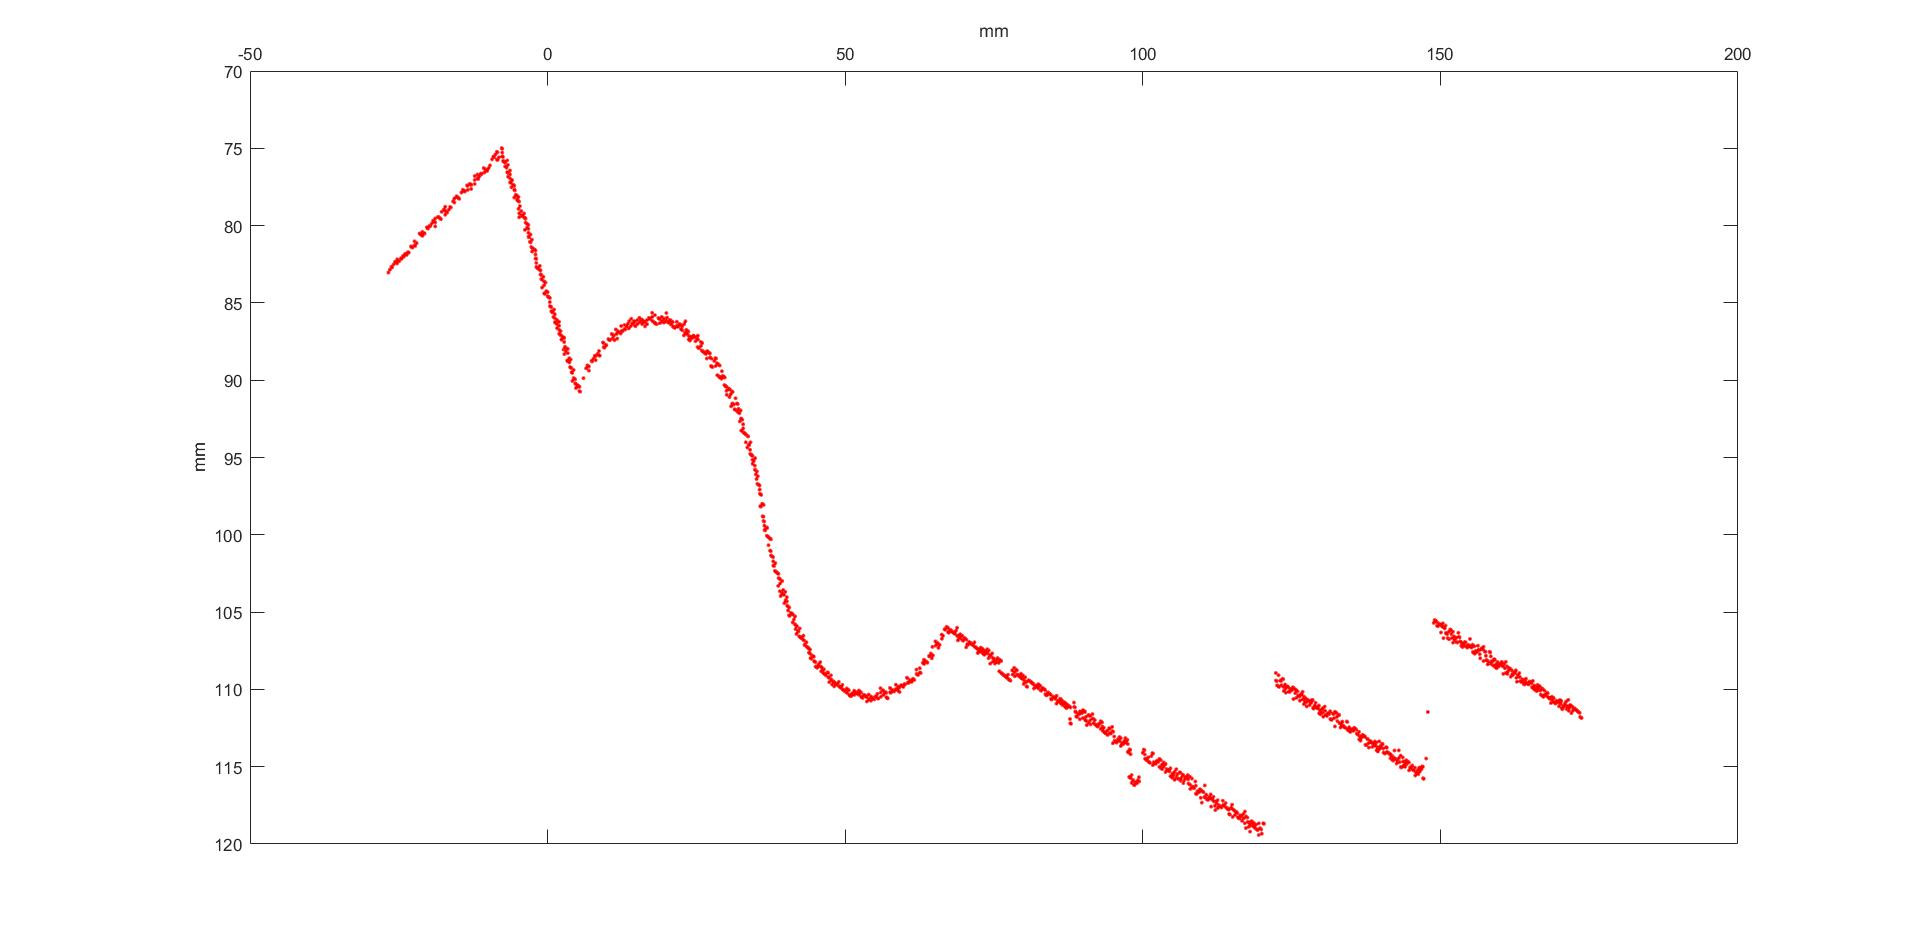
\includegraphics[width=\textwidth]{./images/analysis/t1/pixel_profile_cut.jpg}
    \caption{Laser spots, complete profile}
    \label{fig:c5-profile_pixel}
  \end{minipage}
\end{figure}
\vfill
\begin{figure}
  \centering
  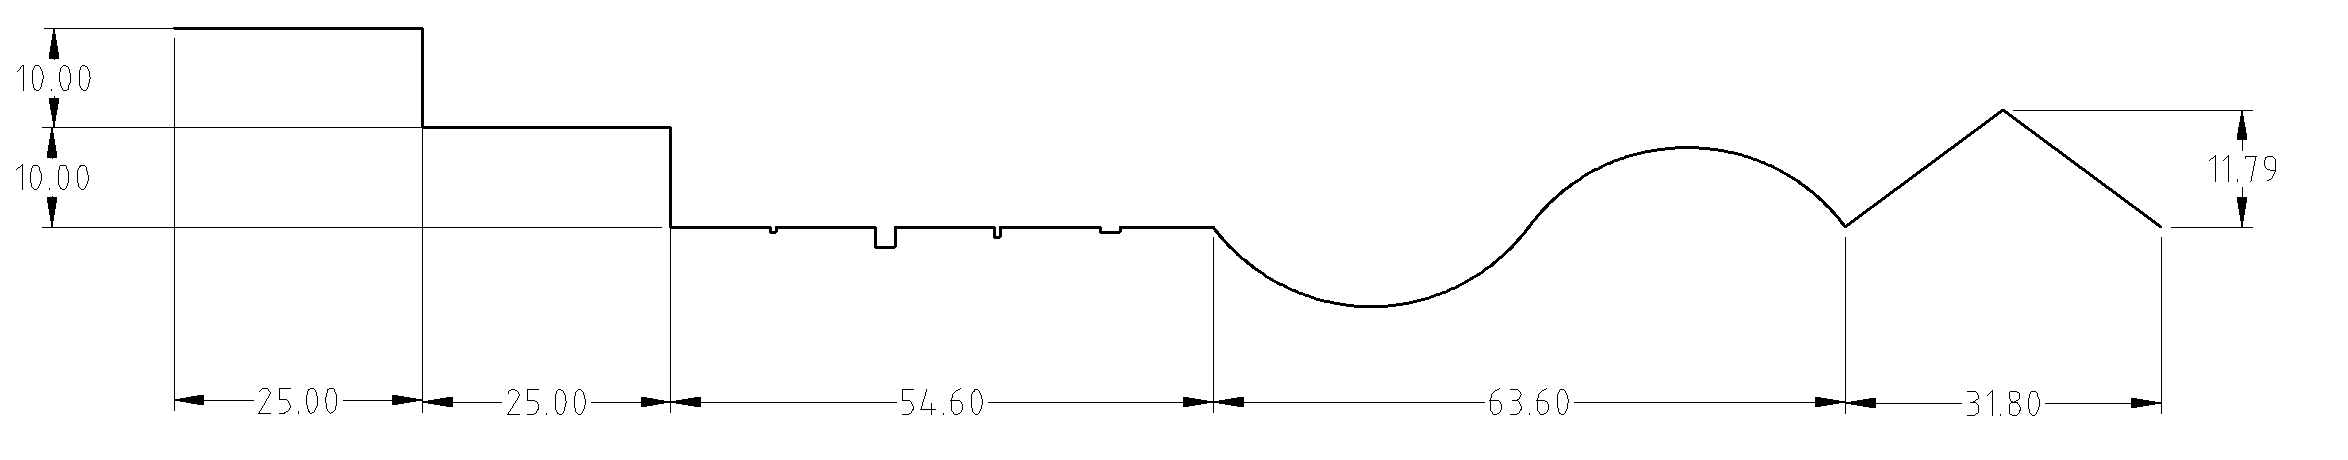
\includegraphics[width=\textwidth]{./images/analysis/t1/cad_misure.png}
  \caption{Measures of the target object}
  \label{fig:c5-cad-misure}
\end{figure}
\vfill
\begin{figure}
  \centering
  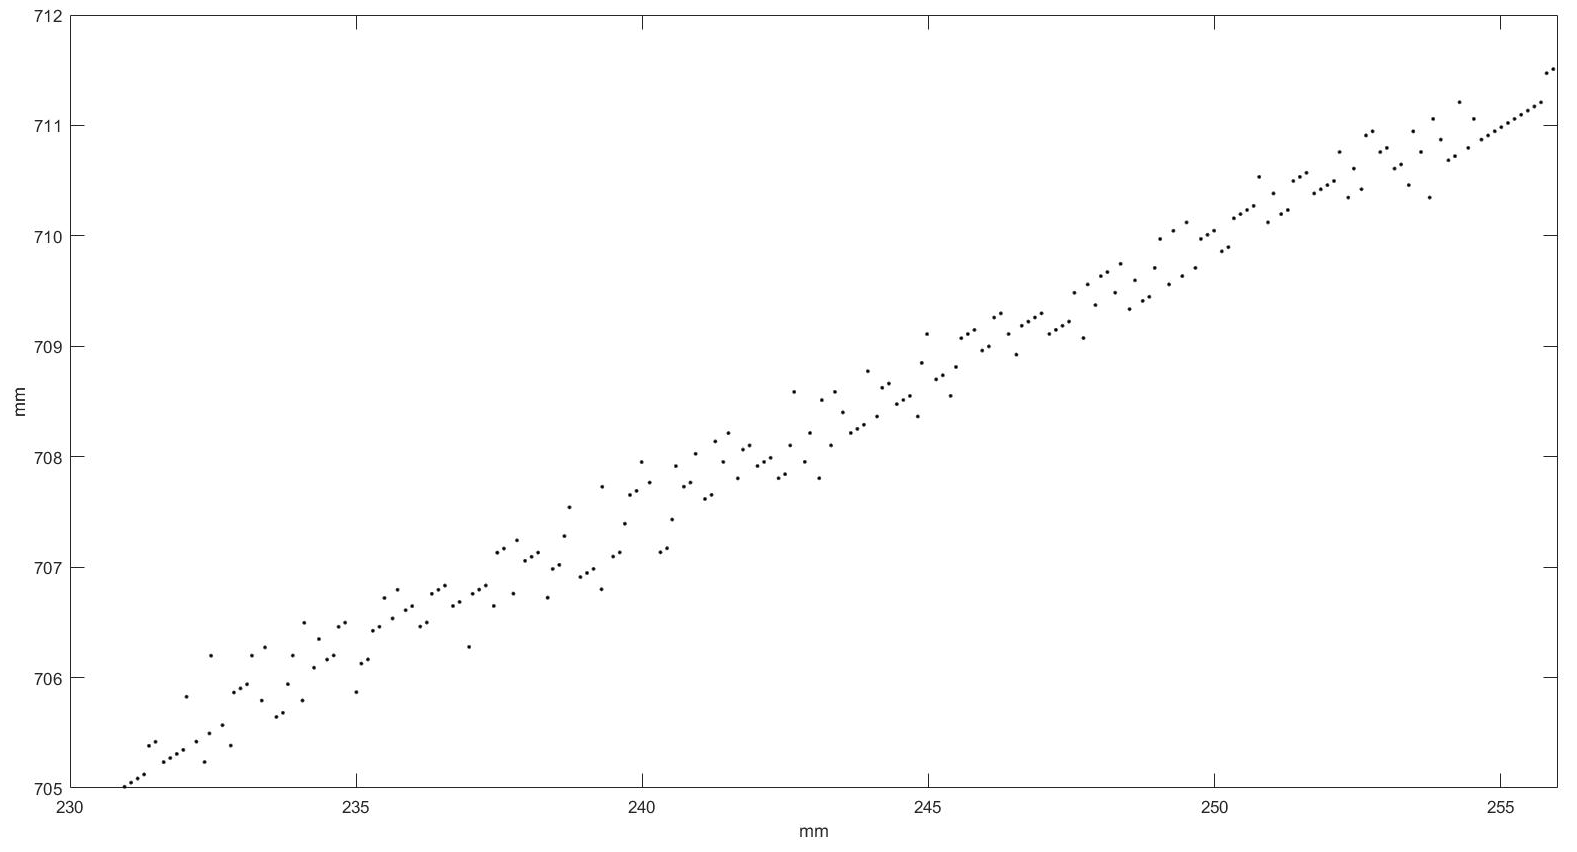
\includegraphics[width=\textwidth]{./images/analysis/t1/pixel_profile_det.jpg}
  \caption{Details of the laser spots}
  \label{fig:c5-profile_pixel_det}
\end{figure}
\vfill
\begin{figure}
  \centering
  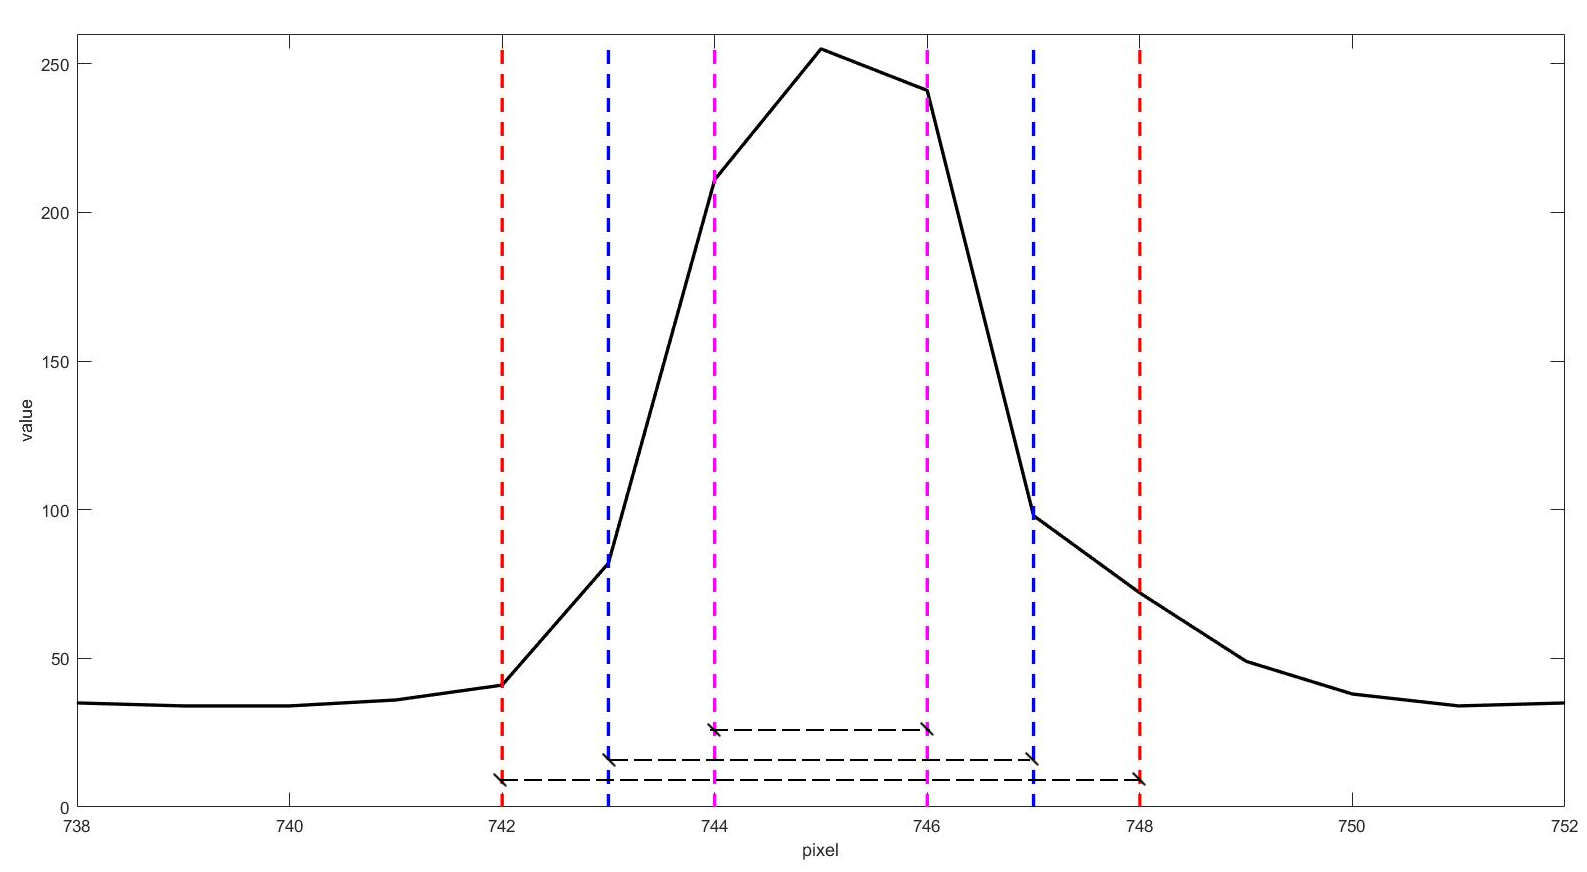
\includegraphics[width=\textwidth]{./images/analysis/t1/peak_distrib.jpg}
  \caption{Distribution of the energy along a row of the image. Vertical lines indicate the 3 windows used.}
  \label{fig:c5-peak_distrib}
\end{figure}
\vfill
\begin{figure}
  \centering
  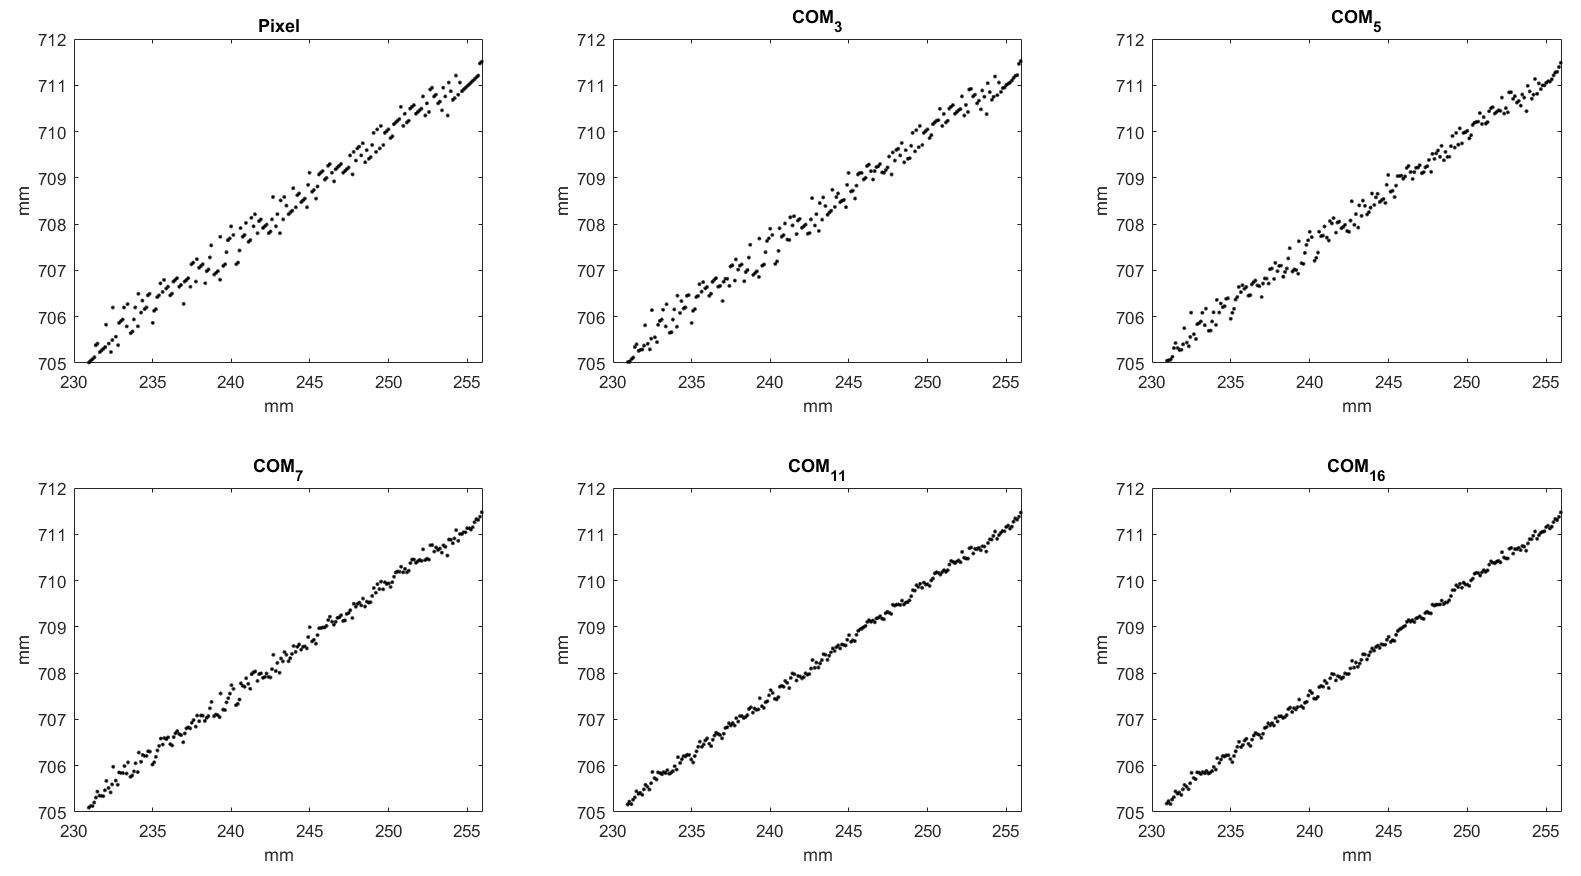
\includegraphics[width=\textwidth]{./images/analysis/t1/com6_cmp.jpg}
  \caption{Comparison of \textit{Center of Mass} applied with extended widow sizes}
  \label{fig:c5-com_cmp_6}
\end{figure}
\vfill
\begin{figure}
  \centering
  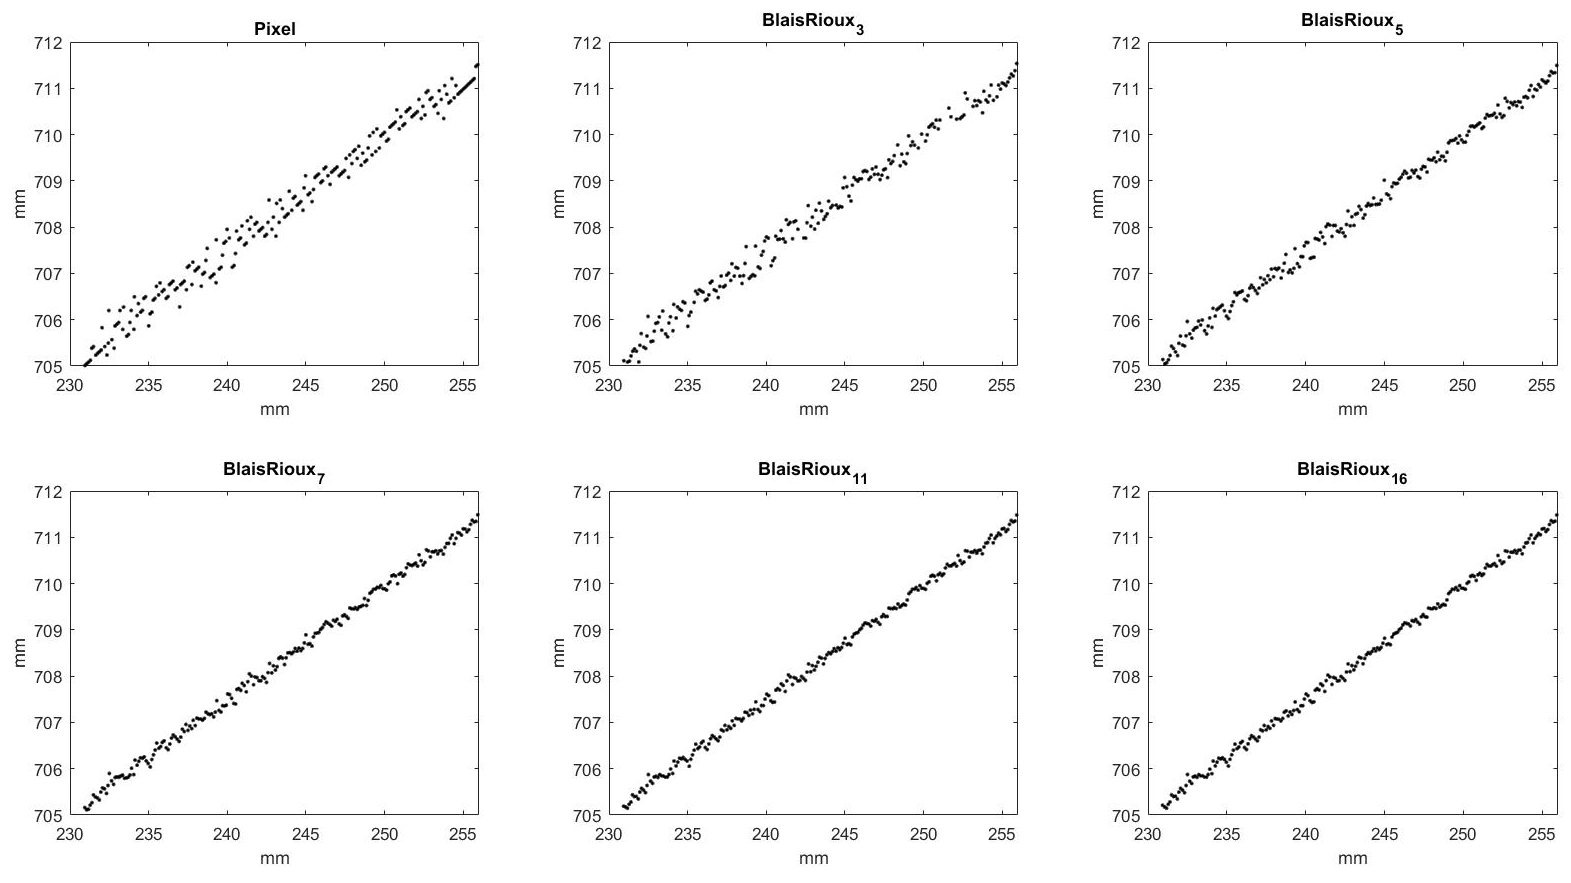
\includegraphics[width=\textwidth]{./images/analysis/t1/br6_cmp.jpg}
  \caption{Comparison of \textit{Blais and Rioux} applied with extended widow sizes}
  \label{fig:c5-br_cmp_6}
\end{figure}
\begin{figure}
  \centering
  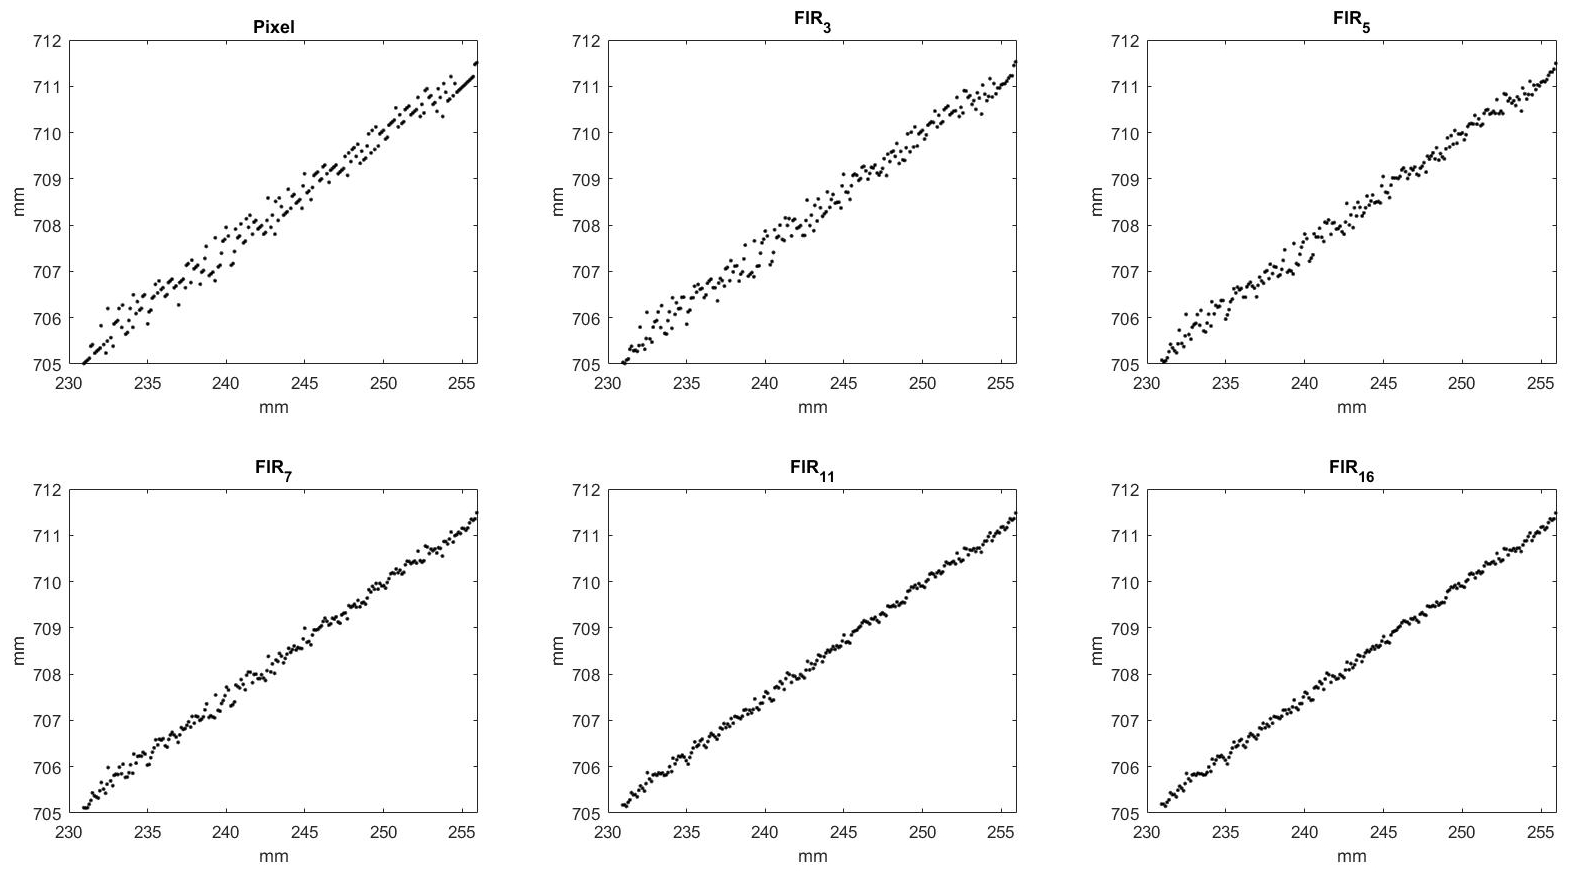
\includegraphics[width=\textwidth]{./images/analysis/t1/fir6_cmp.jpg}
  \caption{Comparison of \textit{FIR} applied with extended widow sizes}
  \label{fig:c5-fir_cmp_6}
\end{figure}
\clearpage

If we magnify the data, as shown in Figure \ref{fig:c5-profile_pixel_det}, we can observe that the acquired profile is very thick. This effect is due to the noise of the laser beam (e.g. speckle), that causes small variations of the positions of the peaks, along a line of the image. Thus, we expected that the use of sub-pixel filters, should reduce the thickness of the beam. All the model described in Section \ref{sec:laser-peaks}, were introduced considering only few pixel around the candidate to be the peak. So we tried to apply them, using windows of $3$, $5$ and $7$ pixel were possible. \\

Unfortunately, the results made us wrong. Observing the live images, we noticed that the width of the Gaussian was on average equal to $20$ pixels, as the row shown in Figure \ref{fig:c5-peak_distrib}: the used interval are too small with respect to signal amplitude. Hence, we decided to increase the window to $11$ and $16$ pixels where possible. In Figure \ref{fig:c5-com_cmp_6} we can see the improvement of the detail shown in Figure \ref{fig:c5-profile_pixel_det}, obtained using the \textit{center of mass}. Therefore, we concluded that, in order to get a sufficiently precise smoothing, it is necessary that the window is bigger enough to contain the whole laser spot. To complete our analysis, we tried to further increase the size of the window. This tests did not lead to significant improvements over the windows of $11$ or $16$ pixels. On the contrary in some cases, for example in noisy areas of the images, or because the background noise, the use of a larger window deteriorated the peak recognition. \\
We reached the same results analysing the remaining filters, as shown in Figures \ref{fig:c5-br_cmp_6} and \ref{fig:c5-fir_cmp_6}. From these observations, we concluded that the windows sizes have to be comparable with the Gaussian: if they are too small, the profile will be less precise; if they are too big, we risk to add noise.

Regarding the remaining filters (Gaussian, Linear and Parabolic), we have found some difficulties extending them, in order to increase the number of points involved in: as we have already said, $3$ pixels are too few to obtain a good approximation of the laser beam. However, this operation has proved to be meaningless. The three models are based on weighted linear models, such that they work properly only if three pixel are used. Change these weights, changes the meaning of the model itself. The only one that has been extended (the Parabolic) did not reach the results reached with the \textit{\acs{COM}}, the \textit{Blaise\&Rioux} or with the \textit{FIR} filter. Thus, we decided to ignore them from our analysis.

A second observation in support of this choice is due to the saturation effect. Sometimes could happen that some consecutive pixels have the same (maximum) value, caused by changing in the illumination of the working place, out of focus lenses or lasers, or caused by translucid or labertian surfaces. If we use only $3$ or $4$ pixels, it is impossible for these filters to properly identify the peak the the laser spot. \\
  
At this point, we were able to evaluate some measures. To simplify the task, we decided to consider a few well-recognizable points of the profile, i.e. the points used in Figure \ref{fig:c5-cad-misure} to add quotes. Thus, we used a simple 3D corner detector, and the measures were computed as differences between the points, after the alignment of the detected profile to the model. \\
Before achieving remarkable results, we found some difficulties. The most important, is related to calibration. As we said in Section \ref{sec:teo-calibration}, it is fundamental that the grid of calibration points covers the entire \acs{FOV} of the camera. Despite that, the points have to be always on focus. If for any reasons this condition is not true, some of these points could affect the quality of the calibration itself. Thus, we manually reduced the grid until we reached a tiny type I error. \\

Finally, we had got the first results. In Figure \ref{fig:c5-match} we shown the match computed before estimate the measures, while in Tables \ref{tab:c5-r1-teo} and \ref{tab:c5-r1-real} we reported an example of how we estimated the measurement error (theoretically and with empirical data), in particular these results are obtained using the \textit{center of mass} with a window of $16$ pixels. Note that, in order to evaluate column \textit{point error}, we assumed that the event that a point falls in $p = (x, y)$ can be modelled as the union of two i.i.d. events, followed by:
  \begin{equation}
    \sigma_p = \sqrt{\sigma_x^2 + \sigma_y^2}
    \label{eq:exp:var-prop}
  \end{equation}
  \begin{figure}[t!]
    \centering
    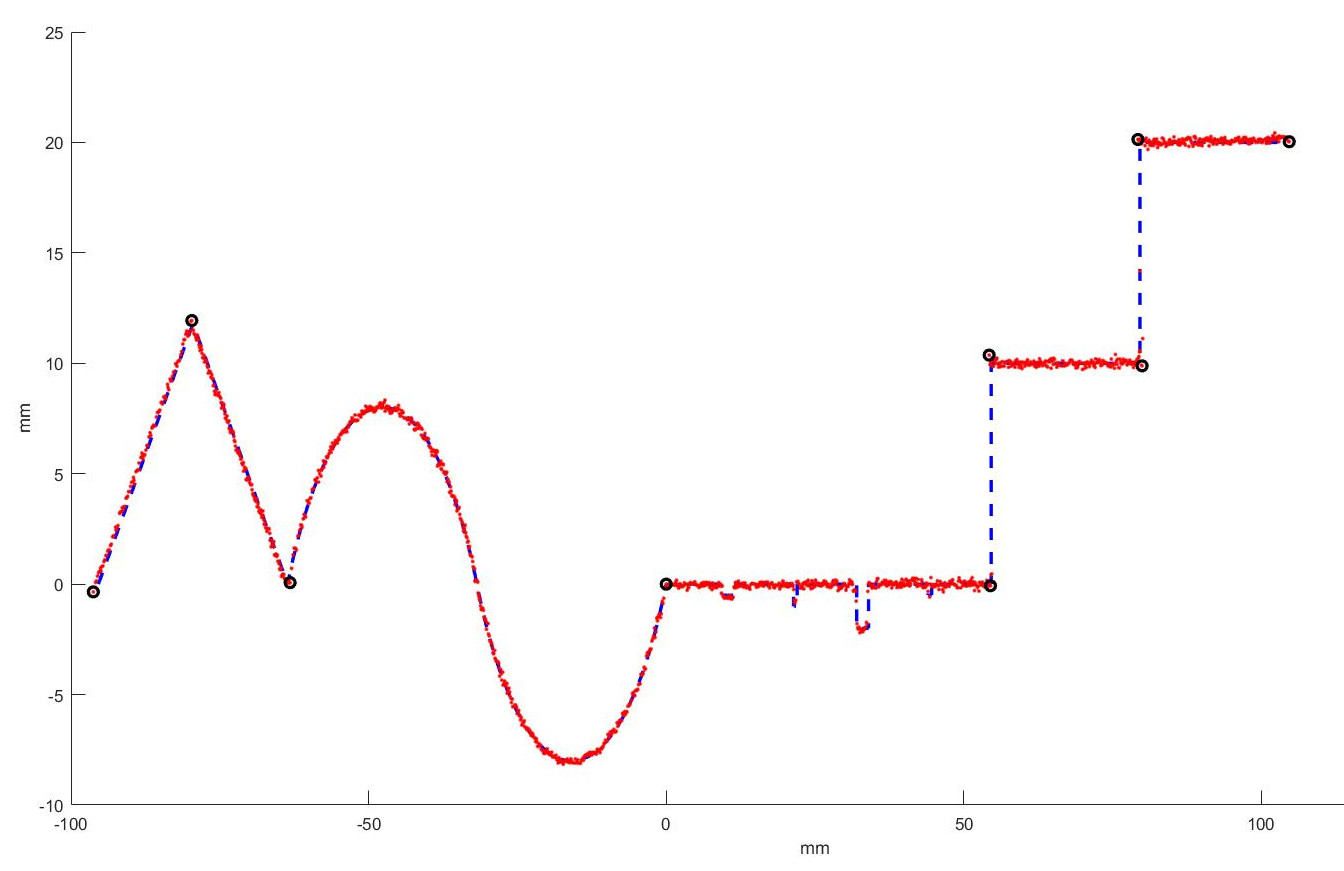
\includegraphics[width=\textwidth]{./images/analysis/t1/example_cut.jpg}
    \caption{Example of match of the profile extracted using \textit{center of mass} with window of $16$ pixel. The model is plotted in blue, while the extracted profile is plotted in red.}
    \label{fig:c5-match}
  \end{figure}
  \begin{table}[b!]
\centering
\begin{tabular}{|r|r|r|r|}
\hline
\multicolumn{1}{|c|}{\textbf{Approximation}} & \multicolumn{1}{c|}{\textbf{Y Error}} & \multicolumn{1}{c|}{\textbf{X Error}} & \multicolumn{1}{c|}{\textbf{Point Error}} \\ \hline
\multicolumn{1}{|c|}{\textit{(pix)}}           & \multicolumn{1}{c|}{\textit{(mm)}}      & \multicolumn{1}{c|}{\textit{(mm)}}      & \multicolumn{1}{c|}{\textit{(mm)}}          \\ \hline
0.1089                                       & 0.0153                                & 0.5678                                & 0.5680                                    \\ \hline
0.1089                                       & 0.0101                                & 0.3261                                & 0.3263                                    \\ \hline
0.1089                                       & 0.0073                                & 0.6246                                & 0.6246                                    \\ \hline
0.1089                                       & 0.0095                                & 0.7877                                & 0.7877                                    \\ \hline
0.1089                                       & 0.0528                                & 0.9875                                & 0.9889                                    \\ \hline
0.1089                                       & 0.0534                                & 0.6900                                & 0.6921                                    \\ \hline
0.1089                                       & 0.1157                                & 0.8070                                & 0.8152                                    \\ \hline
0.1089                                       & 0.1172                                & 0.4760                                & 0.4902                                    \\ \hline
0.1089                                       & 0.2220                                & 0.5741                                & 0.6155                                    \\ \hline
\multicolumn{3}{|r|}{\textbf{Mean}}                                                                                          & \textbf{0.6565}                           \\ \hline
\end{tabular}
\caption{Theoretical results obtained using the \textit{Center of Mass} with window of 16 pixel}
\label{tab:c5-r1-teo}
\end{table}
  \begin{table}[h!]
\centering
\begin{tabular}{|r|r|r|r|r|r|r|}
\hline
\multicolumn{3}{|c|}{\textbf{Abscissa}}                                                                             & \multicolumn{3}{c|}{\textbf{Ordinate}}                                                                             & \multicolumn{1}{c|}{\multirow{2}{*}{\textbf{Point Error}}} \\ \cline{1-6}
\multicolumn{1}{|c|}{\textbf{Model}} & \multicolumn{1}{c|}{\textbf{Profile}} & \multicolumn{1}{c|}{\textbf{Errors}} & \multicolumn{1}{c|}{\textbf{Model}} & \multicolumn{1}{c|}{\textbf{Profile}} & \multicolumn{1}{c|}{\textbf{Errors}} & \multicolumn{1}{c|}{}                                      \\ \hline
\multicolumn{1}{|c|}{\textit{(mm)}}           & \multicolumn{1}{c|}{\textit{(mm)}}      & \multicolumn{1}{c|}{\textit{(mm)}}      & \multicolumn{1}{c|}{\textit{(mm)}} & \multicolumn{1}{c|}{\textit{(mm)}}      & \multicolumn{1}{c|}{\textit{(mm)}}      & \multicolumn{1}{c|}{\textit{(mm)}}          \\ \hline
15.9010                              & 16.5450                               & 0.6438                               & 11.7920                             & 12.2720                               & 0.4804                               & 0.8033                                                     \\ \hline
15.9000                              & 16.5160                               & 0.6157                               & 11.7920                             & 11.8430                               & 0.0511                               & 0.6178                                                     \\ \hline
63.6000                              & 63.1840                               & 0.4159                               & 0.0000                              & 0.0909                                & 0.0909                               & 0.4257                                                     \\ \hline
54.6000                              & 54.4860                               & 0.1144                               & 0.0000                              & 0.0863                                & 0.0863                               & 0.1433                                                     \\ \hline
0.0000                               & 0.2235                                & 0.2235                               & 10.0000                             & 10.4530                               & 0.4530                               & 0.5051                                                     \\ \hline
25.0000                              & 25.6950                               & 0.6949                               & 0.0000                              & 0.5067                                & 0.5067                               & 0.8600                                                     \\ \hline
0.0000                               & 0.7019                                & 0.7019                               & 10.0000                             & 10.2750                               & 0.2746                               & 0.7537                                                     \\ \hline
25.0000                              & 25.4190                               & 0.4189                               & 0.0000                              & 0.1010                                & 0.1010                               & 0.4309                                                     \\ \hline
\multicolumn{6}{|r|}{\textbf{Mean}}                                                                                                                                                                                                      & \textbf{0.5675}                                            \\ \hline
\end{tabular}
\caption{Results obtained using the \textit{Center of Mass} with window of 16 pixel}
\label{tab:c5-r1-real}
\end{table}

In Table \ref{tab:c5-r1-all}, instead, we have summarized the results obtained with all the filters considered. As we can see, they are significantly higher than the $0.1 \, mm$ that we wanted to reach. However, some considerations can already be made.
  \begin{table}[t!]
\centering
\begin{tabular}{|c|c|r|r|r|}
\hline
\textbf{\textbf{Error}}  & \multicolumn{1}{l|}{\textbf{Window}} & \multicolumn{2}{c|}{\textbf{Theoretical}}                                & \multicolumn{1}{c|}{\textbf{Empirical}} \\ \hline
\textit{}                   & \textit{}                            & \multicolumn{1}{c|}{\textit{(pix)}}       & \multicolumn{1}{c|}{\textit{(mm)}}        & \multicolumn{1}{c|}{\textit{(mm)}}      \\ \hline
\textit{\textbf{Pixel}} & 1                                    & 0.2887                                    & 0.6579                                    & 0.6764                                  \\ \hline
\textit{\textbf{COM}}   & 16                                   & 0.1089                                    & 0.6565                                    & 0.5675                                  \\ \hline
\textit{\textbf{COM}}   & 20                                   & 0.0921                                    & 0.6565                                    & 0.5628                                  \\ \hline
\textit{\textbf{BR}}    & 16                                   & 0.1498                                    & 0.6596                                    & 0.5365                                  \\ \hline
\textit{\textbf{BR}}    & 20                                   & 0.1471                                    & 0.6558                                    & 0.3263                                  \\ \hline
\textit{\textbf{FIR}}   & 16                                   & 0.1671                                    & 0.6564                                    & 0.3654                                  \\ \hline
\end{tabular}
\caption{Summary of the results obtained with the filters used.}
\label{tab:c5-r1-all}
\end{table}
  
First of all, it is clear that all the proposed filters increase the precision of the spot localization. Then, it seems that the assumptions made in Section \ref{sec:laser-peaks} about the performances of the filters, are not complete: from a mathematical point of view, the \textit{center of mass} is better; however, in real case, the \textit{Blais\&Rioux} and the \textit{FIR} gave better results.

The second thing to consider, is the quality of the optical bench:
  \begin{itemize}
    \item The laser wasn't good enough, it was too thick and affected by noise. We did several attempts to properly set the properties of the camera, in order to reduce the amount of light collected by the sensor, i.e. reduce the width of the collected laser beam. Nevertheless, the thickness of the resulting profile is about $0.1 \, mm$.
    \item The model wasn't well defined. Many parameters, such as the error of the Scheimpfulg angles, or the error made positioning the laser projector, weren't known.
  \end{itemize}
Regarding this last point, we understood that the parameters not estimated by the model, can be defined in two different ways: on the one hand they strongly depends by the system itself, and by how good it is build; on the other, they allow to evaluate how good it must be made to reach the precision proposed by the model. Thus, in this first experiment, the model was tuned to reach the results empirically obtained, instead that the contrary. \\

All the imprecisions and the found problems, suggested us to use a more precise and well built systems to evaluate the correctness of our model.
